\section{Occurrence projection and dormant arithmetic structure}\label{sec:occurrence}
The second projection sends a state to its occurrence set. For integers it has a direct generative meaning.

\begin{proposition}[\SIV{2}: occurrence projection and primitive-relation information]\label{prop:P2}\status{new, proved; (b),(c) cited}
\begin{enumerate}[label=(\alph*),itemsep=1pt]
\item \emph{Occurrences are incoming steps.} For an integer $t\ge1$ the map $d\mapsto(N,m)=\bigl(d-1,\ t(d-1)/d^2\bigr)$ is a bijection from $D(t)$ onto the set of generative steps $m\xrightarrow{N}t$. Consequently $|D(t)|$ is the in-degree of $t$, and for every $m_0$ the number $H(m_0,t)$ of histories from $m_0$ to $t$ satisfies $H(m_0,t)=\sum_{d\in D(t)}H\bigl(m_0,\ t(d-1)/d^2\bigr)$ (with $H(m_0,m_0)=1$ and the convention that terms with $t(d-1)/d^2<m_0$ vanish). Moreover $N+1\in D(T_N(m))$ for every admissible step.
\item \emph{Factorization.} The realised fibre, $\Kmove(x)$ and all its derived data factor through $x\mapsto D(x)$; for integer $t$ the whole record is a function of $\max D(t)$ (\Src{III}{thm:R3T1a}, \Src{III}{thm:B2T1}).
\item \emph{Obstruction.} The primitive relation system does not factor through $D$: for primes $r\ge13$, $r\equiv5\pmod8$, the states $x_r=25r^2/(5r-1)$ and $y_r=25r^2/8$ have $D(x_r)=D(y_r)=\{5r\}$ and the same active primes and box, but $|\Gr(x_r)|=2$ and $|\Gr(y_r)|=4$ (\Src{III}{thm:R3T1}(i)).
\end{enumerate}
\end{proposition}
\begin{proof}
(a) If $m\xrightarrow{N}t$ then $t=m(N+1)^2/N$ with $N\mid m$; we have $tN=m(N+1)^2$, so $(N+1)^2\mid tN$, and $\gcd(N,N+1)=1$ gives $(N+1)^2\mid t$, i.e.\ $d=N+1\in D(t)$ (here $d\ge2$), and $m=tN/(N+1)^2=t(d-1)/d^2$. Conversely if $d\in D(t)$ put $N=d-1$ and $m=t(d-1)/d^2$; then $m\in\Z$ because $d^2\mid t$, $N\mid m$ because $m=(t/d^2)N$, and $T_N(m)=m(N+1)^2/N=t$. The two assignments are inverse. A history to $t$ is a history to the predecessor $m$ followed by the step to $t$, which gives the recursion. For the last statement $(N+1)^2\mid m(N+1)^2/N=T_N(m)$ because $N\mid m$ makes $m/N$ an integer.
(b) and (c) are the cited theorems; for (c) we recomputed $D(x_{13})=D(y_{13})=\{65\}$ (Appendix~\ref{app:finite}).
\end{proof}
\begin{corollary}\label{cor:P2}
The occurrence set of an integer is the branching set of its ancestry: histories to $t$ are sequences of choices of elements of $D$ along the way. Hence the invariant counting histories depends on $t$ through the recursion above, not through $D(t)$ alone (compare \cref{prop:P5}).
\end{corollary}
\paragraph{Information chain.} Combining \cref{prop:P2} with \cref{prop:P1}: the chain $\mathrm{Hist}\to\mathrm{Cls}\to\mathrm{Cont}\to\Z\to\{D\}\to\{\Kmove\}\to\{\beta\}$ consists of surjections, each a factorization of the next by \cref{lem:factor}; the first three arrows lose information on every set containing the witnesses of \cref{prop:P1}; the fourth, $t\mapsto D(t)$, is non-injective (all $t$ with the same square-divisor set, \cref{prop:P5}); and $D\mapsto\Gr$ does not exist at all (\cref{prop:P2}(c)). \cref{fig:fact} shows the chain with the status of each arrow.
\begin{figure}[t]\centering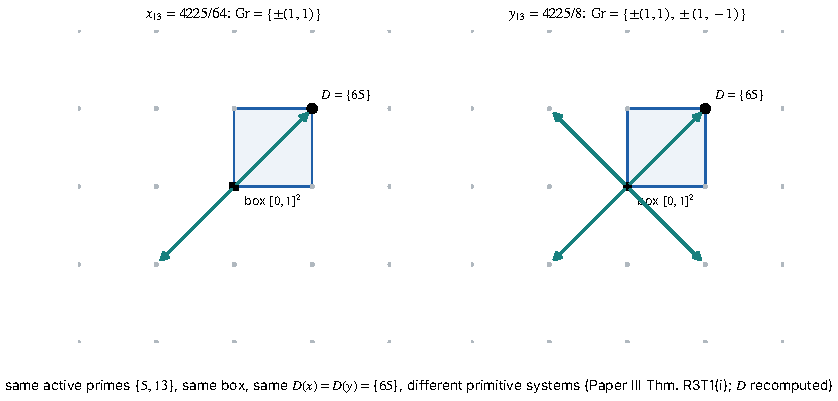
\includegraphics[width=\linewidth]{fig06_equalD_diffGr.pdf}
\caption{\textbf{Occurrence projection and dormant relations.} The states $x_{13}=4225/64$ and $y_{13}=4225/8$ have the same occurrence set $\{65\}$, the same active primes $\{5,13\}$ and the same box $[0,1]^2$, but the primitive systems differ: the extra pair $\pm(1,-1)$ is a primitive relation of $y_{13}$ that is not realised at $x_{13}$. \emph{Exact data of \Src{III}{thm:R3T1}(i) with $r=13$; $D$ recomputed; the lattice pictures are schematic.}}\label{fig:equalD}\end{figure}
